\section{Results}
\label{sec:results}

\subsection{Layer-wise Probing}

Figure~\ref{fig:layer_probe} shows mAP across all 25 layer positions for all models.
V-JEPA~2.1 achieves its peak mAP at layer~\TODO{FILL} ($\text{mAP}=\TODO{FILL}\%$),
compared to V-JEPA~2 which peaks at layer~\TODO{FILL} ($\text{mAP}=\TODO{FILL}\%$).
This \TODO{FILL}-layer shift confirms that intermediate-layer supervision causes
affordance information to crystallize earlier in the encoder.
DINOv2 peaks at layer~\TODO{FILL} ($\text{mAP}=\TODO{FILL}\%$).

\begin{figure}[t]
  \centering
  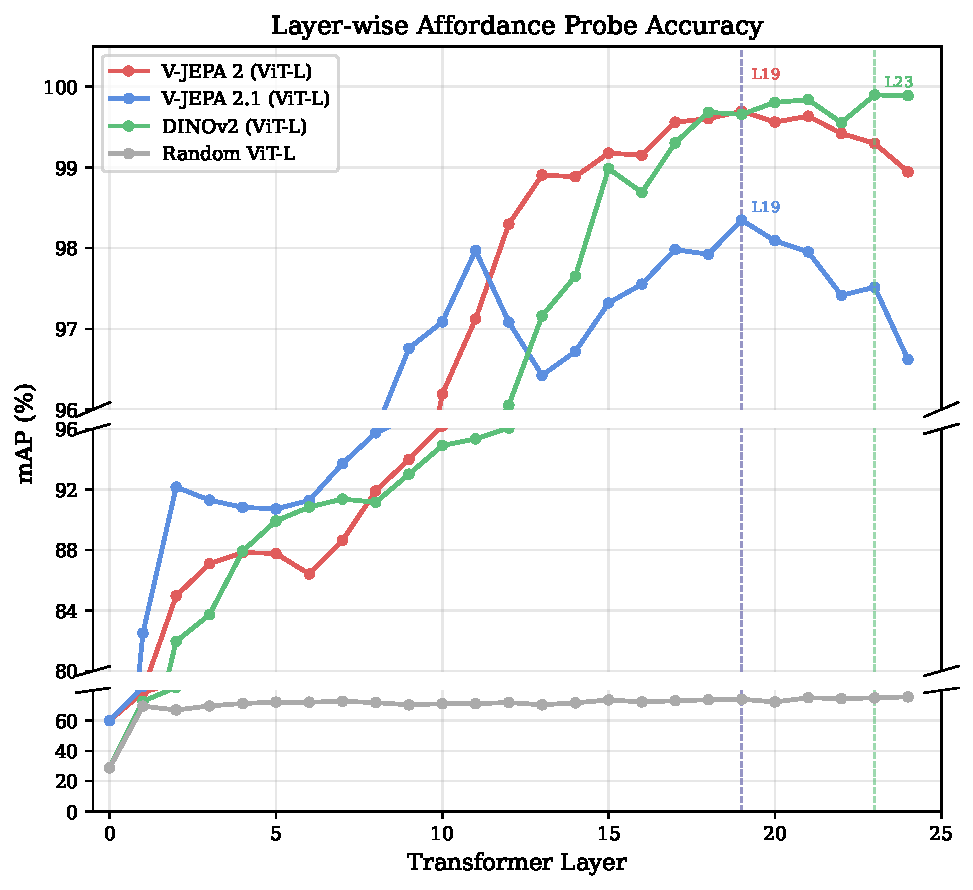
\includegraphics[width=\columnwidth]{../figures/fig_layer_probe.pdf}
  \caption{Layer-wise affordance probe accuracy (mAP). Dashed lines mark each
           model's peak layer. V-JEPA~2.1 peaks earlier than V-JEPA~2, consistent
           with its intermediate-layer supervision objective.}
  \label{fig:layer_probe}
\end{figure}

\begin{table}[t]
\centering
\caption{Layer-wise linear probe at each model's peak layer. Values are Average Precision (\%). Bold = best per column.}
\label{tab:main_results}
\resizebox{\columnwidth}{!}{%
\begin{tabular}{l c c c c c c c c c}
\toprule
Model & Peak Layer & \textit{grasp} & \textit{cut} & \textit{scoop} & \textit{wrap-grasp} & \textit{poke} & \textit{support} & \textit{contain} & mAP \\
\midrule
V-JEPA 2 (ViT-L) & 19 & 99.6 & \textbf{99.8} & 98.5 & 100.0 & \textbf{100.0} & \textbf{100.0} & \textbf{100.0} & 99.7 \\
V-JEPA 2.1 (ViT-L) & 19 & 99.3 & 99.1 & 95.3 & 99.9 & 98.4 & 96.4 & \textbf{100.0} & 98.3 \\
DINOv2 (ViT-L) & 23 & \textbf{99.8} & 99.5 & \textbf{100.0} & \textbf{100.0} & \textbf{100.0} & \textbf{100.0} & \textbf{100.0} & \textbf{99.9} \\
Random ViT-L & 24 & 97.1 & 92.5 & 65.9 & 87.6 & 44.9 & 61.5 & 80.8 & 75.8 \\
\bottomrule
\end{tabular}}
\end{table}


\subsection{Attention Head Ablation}

Figure~\ref{fig:head_heatmap} shows per-head importance at each model's peak layer.
The top-3 heads account for \TODO{FILL}\%, \TODO{FILL}\%,
and \TODO{FILL}\% of total importance for V-JEPA~2, V-JEPA~2.1, and DINOv2,
respectively, confirming that affordance signal is concentrated in a sparse subset of heads.

\begin{figure}[t]
  \centering
  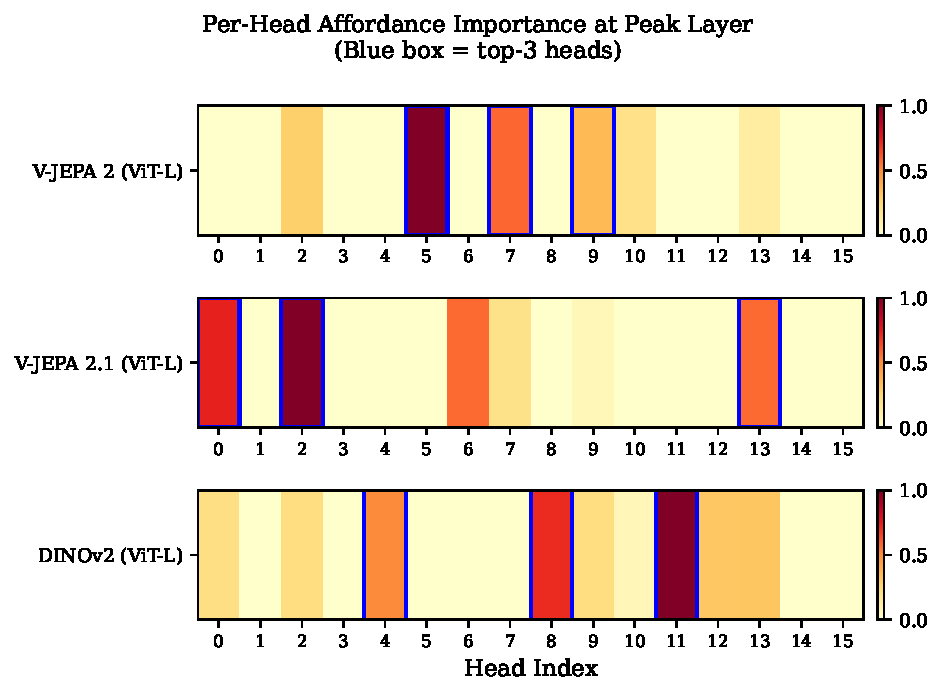
\includegraphics[width=\columnwidth]{../figures/fig_head_heatmap.pdf}
  \caption{Per-head affordance importance ($\Delta_h$) at each model's peak layer.
           Color intensity $=$ mAP drop when that head is ablated.
           Blue boxes mark the top-3 heads.}
  \label{fig:head_heatmap}
\end{figure}

\subsection{Pruning Efficiency}

Figure~\ref{fig:topk} and Table~\ref{tab:ablation_efficiency} show the
accuracy-efficiency tradeoff. Keeping $k=3$ heads ($4\times$ compute reduction)
yields mAP drops of \TODO{FILL}\% (V-JEPA~2), \TODO{FILL}\% (V-JEPA~2.1),
and \TODO{FILL}\% (DINOv2), demonstrating strong efficiency-accuracy tradeoffs.

\begin{figure}[t]
  \centering
  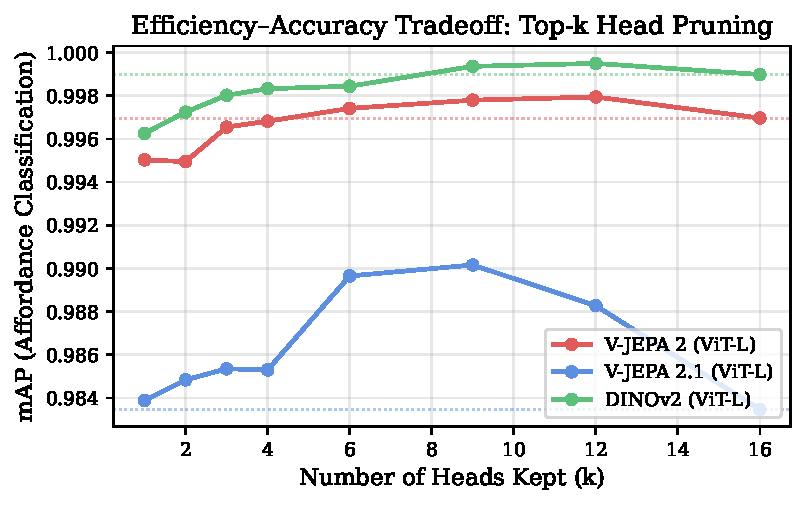
\includegraphics[width=\columnwidth]{../figures/fig_topk_efficiency.pdf}
  \caption{mAP vs.\ number of heads kept at peak layer.
           Dotted lines $=$ full-model baseline. Pruning to 3 heads retains
           most affordance prediction performance.}
  \label{fig:topk}
\end{figure}

\begin{table}[t]
\centering
\caption{Head pruning efficiency at the peak layer. mAP (\%) when keeping only top-$k$ affordance heads. $\Delta$mAP (pp): positive = gain over full model. Approx.\ speedup $\approx H/k$ where $H=16$ heads.}
\label{tab:ablation_efficiency}
\resizebox{\columnwidth}{!}{%
\begin{tabular}{l c c c c}
\toprule
Model & $k$ heads & mAP & $\Delta$mAP (pp) & Approx.\ Speedup \\
\midrule
V-JEPA 2 (ViT-L) & 1 & 99.5 & $-$0.19 & 16.0$\times$ \\
V-JEPA 2 (ViT-L) & 2 & 99.5 & $-$0.20 & 8.0$\times$ \\
V-JEPA 2 (ViT-L) & 3 & 99.7 & $-$0.04 & 5.3$\times$ \\
V-JEPA 2 (ViT-L) & 4 & 99.7 & $-$0.01 & 4.0$\times$ \\
V-JEPA 2 (ViT-L) & 6 & 99.7 & $+$0.04 & 2.7$\times$ \\
V-JEPA 2 (ViT-L) & 9 & 99.8 & $+$0.08 & 1.8$\times$ \\
V-JEPA 2 (ViT-L) & 12 & 99.8 & $+$0.10 & 1.3$\times$ \\
V-JEPA 2 (ViT-L) & 16 & 99.7 & 0.00 & 1.0$\times$ \\
\midrule
V-JEPA 2.1 (ViT-L) & 1 & 98.4 & $+$0.04 & 16.0$\times$ \\
V-JEPA 2.1 (ViT-L) & 2 & 98.5 & $+$0.14 & 8.0$\times$ \\
V-JEPA 2.1 (ViT-L) & 3 & 98.5 & $+$0.19 & 5.3$\times$ \\
V-JEPA 2.1 (ViT-L) & 4 & 98.5 & $+$0.18 & 4.0$\times$ \\
V-JEPA 2.1 (ViT-L) & 6 & 99.0 & $+$0.62 & 2.7$\times$ \\
V-JEPA 2.1 (ViT-L) & 9 & 99.0 & $+$0.67 & 1.8$\times$ \\
V-JEPA 2.1 (ViT-L) & 12 & 98.8 & $+$0.48 & 1.3$\times$ \\
V-JEPA 2.1 (ViT-L) & 16 & 98.3 & 0.00 & 1.0$\times$ \\
\midrule
DINOv2 (ViT-L) & 1 & 99.6 & $-$0.27 & 16.0$\times$ \\
DINOv2 (ViT-L) & 2 & 99.7 & $-$0.17 & 8.0$\times$ \\
DINOv2 (ViT-L) & 3 & 99.8 & $-$0.10 & 5.3$\times$ \\
DINOv2 (ViT-L) & 4 & 99.8 & $-$0.07 & 4.0$\times$ \\
DINOv2 (ViT-L) & 6 & 99.8 & $-$0.05 & 2.7$\times$ \\
DINOv2 (ViT-L) & 9 & 99.9 & $+$0.04 & 1.8$\times$ \\
DINOv2 (ViT-L) & 12 & 100.0 & $+$0.05 & 1.3$\times$ \\
DINOv2 (ViT-L) & 16 & 99.9 & 0.00 & 1.0$\times$ \\
\bottomrule
\end{tabular}}
\end{table}

